%%%%%%%%%%%%%%%%%%%%%%%%%%%%%%%%%%%%%%%%%%%%%%%%%%%%
\documentclass[fleqn,10pt,twocolumn]{SICE14}
\usepackage{epstopdf}
\usepackage{amsmath}
\usepackage{cite}
\usepackage{multirow}
\title{Implementation of Genetic Network Programming and Knapsack Problem for Record Clustering on Distributed Database }

\author{Wirarama Wedashwara${}^{\dagger}$, Shingo Mabu, Masanao Obayashi and Takashi Kuremoto}
% The dagger symbol indicates the presenter.
\speaker{Wirarama Wedashwara}

\affils{Graduate School of Science and Engineering, Yamaguchi University, Yamaguchi, Japan\\
(Tel: +81 83-933-5000; E-mail: t001we@yamaguchi-u.ac.jp)\\
}
\abstract{%
This research involves implementation of genetic network programming (GNP) and knapsack problem (KP) to solve record clustering on distributed databases. The objective is to distribute big data to certain sites with the limited amount of capacities by considering the similarity of distributed data in each site. GNP is used to extract rules from big data by considering characteristics (value ranges) of each attribute in a dataset. 
KP is used to distribute rules to each site by considering similarity (value) and data amount (weight) related to each rule to match the site capacities.
}

\keywords{%
Genetic Network Programming, Database Clustering, Knapsack Problem, Record Clustering
}

\begin{document}

\maketitle

%-----------------------------------------------------------------------

\section{Introduction}

Distributed database management system (DDBMS) could be a solution for large scale information systems with large amount of data growth and data accesses. DDBMS is recently used in online service websites such as online shops and social networking services that are openly accessible by world wide users.

A distributed database (DDB) is a collection of data that logically belongs to the same system but is spread over the sites of a computer network (Fig. \ref{ddbms}). A DDBMS is then defined as a software system that permits the management of DDB and makes the distribution of data between databases and software transparent to the users \cite{recordclustering}.

Fragmentation is a design technique to divide a single relation or class of a database into two or more partitions such that the combination of the partitions provides the original database without any loss of information. This reduces the amount of irrelevant data accessed by the applications of the database, thus reducing the number of disk accesses \cite{horizontalfragmentation,horizontalfragmentation2}.

DDBMS fragment problems contain the following elements.
\begin{description}
\item[Database Structure:] How a global relation should be fragmented?
\item[Database Content:] What the necessary information for fragmentation and allocation is?
\item[Storage Capacity:] How fragments should be allocated to the sites with the limited capacities in the network?
\item[Replication:] How many copies of a fragment should be replicated? 
\end{description}

Objective of this research is to realize record clustering or horizontal fragmentation. Record clustering allows to find a relation or class to be partitioned into disjoint tuples or instances. Intuition behind horizontal fragmentation is that every site should hold all information that is used to answer queries and the information in the site should be fragmented so the queries of the site run faster. 

The objective of the fragmentation is to create fragments of data, distribute them into several sites which have different capacities, and distributed fragments should match with the capacity of each site.

In this paper, a novel method combining genetic network programming (GNP) and knapsack problem for fragment allocation is proposed. Hypothesis of this research are the implementation of GNP for data mining can create effective fragments from complicated dataset and KP can handle the problem of distributing fragments to several sites considering value (similarity of data) and mass (data size) in DDBMS. Therefore, it could be a solution to the fragment allocation and site storage capacity problems.

\begin{figure}[tb]
\begin{center}
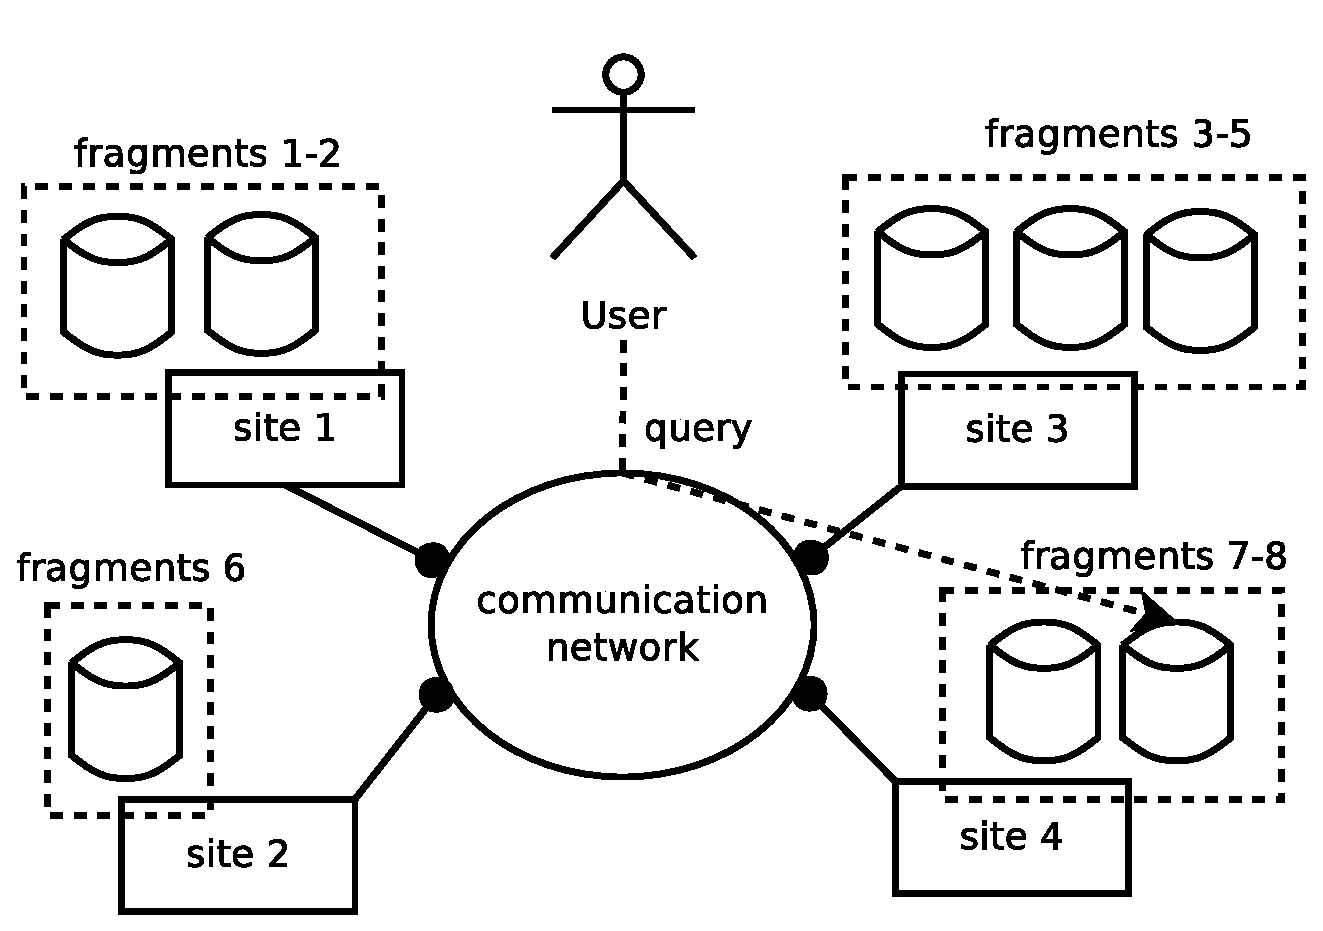
\includegraphics[width=8cm]{ddbms}
\caption{\label{ddbms} A distributed database environment}
\end{center}
\end{figure}

This paper is organized as follows. Section 2 describes a review of the proposed framework, section 3 describes the detailed algorithm of the proposed framework, section 4 shows the simulation results, and finally section 5 is devoted to conclusions.

\begin{table}[tb]
\caption{\label{frequency-table}Example of Frequency Table of Price Attribute}
%\begin{flushleft}
\begin{tabular}{|l|l|l|l|l|l|}
\hline 
$x$ & $f$ & $xf$ & $(x-\overline{x})$ & $(x-\overline{x})^{2}$ & $(x-\overline{x})^{2}f$\tabularnewline
\hline 
10 & 30 & 300 & -65.42 & 4279.34 & 128380.21\tabularnewline
\hline 
25 & 25 & 625 & -50.42 & 2541.84 & 63546.01\tabularnewline
\hline 
50 & 20 & 1000 & -25.42 & 646.01 & 12920.14\tabularnewline
\hline 
80 & 140 & 11200 & 4.58 & 21.01 & 2940.97\tabularnewline
\hline 
100 & 65 & 6500 & 24.58 & 604.34 & 39282.12\tabularnewline
\hline 
150 & 20 & 3000 & 74.58 & 5562.67 & 111253.47\tabularnewline
\hline 
Total & 300 & 22625 &  &  & 358322.92\tabularnewline
\hline 
\end{tabular}
%\par\end{flushleft}
\end{table}

\section{Review of the Proposed Framework}

\subsection{Genetic Network Programming}
GNP is an evolutionary optimization technique, which uses directed graph structures instead of strings in genetic algorithm or trees in genetic programming, which leads to enhancing the representation ability with compact programs derived from the re-usability of nodes in a graph structure.

In GNP, nodes are interpreted as minimum units of the agent’s judgment and action. Sequences are represented by connecting nodes in a graph structure. GNP does not return to the start node when the actions are completed. The next judgment and action are always influenced by the previous ones. Judgment and processing by a GNP program are performed on the node level. 

The basic structure of GNP is illustrated in Fig. \ref{gnpbasic}, with S denoting the start node. There are two kinds of nodes, judgment nodes and processing nodes, with judgment $J_{p}$ and processing $P_{q}$ respectively assigned. $J_{p}$ (p = 1, . . . , n) denotes the p-th judgment, stored in a library for judgment nodes, while $P_{q}$ (q = 1, . . . , m) denotes the q-th processing, stored in a library for processing nodes \cite{gnp1, gnp2}. 

In implementation of data mining, judgement node represents attributes of dataset. Judgement represents a support/suitability of record on dataset to the value of each judgement node. Processing nodes replaced randomly pointed to sequence of judgement nodes and processed sequentially by its index. Only judgement nodes which pointed by processing nodes will be proccesed as rule. For example in Fig. \ref{gnpdatamining} there is a three processing nodes and five judgement nodes. Pointed judgement nodes are $\{A1,B2,C1\}$, so extracted rule represent all record on dataset that supports value of $A1 \cap B2 \cap C1$.

\begin{figure}[tb]
\begin{center}
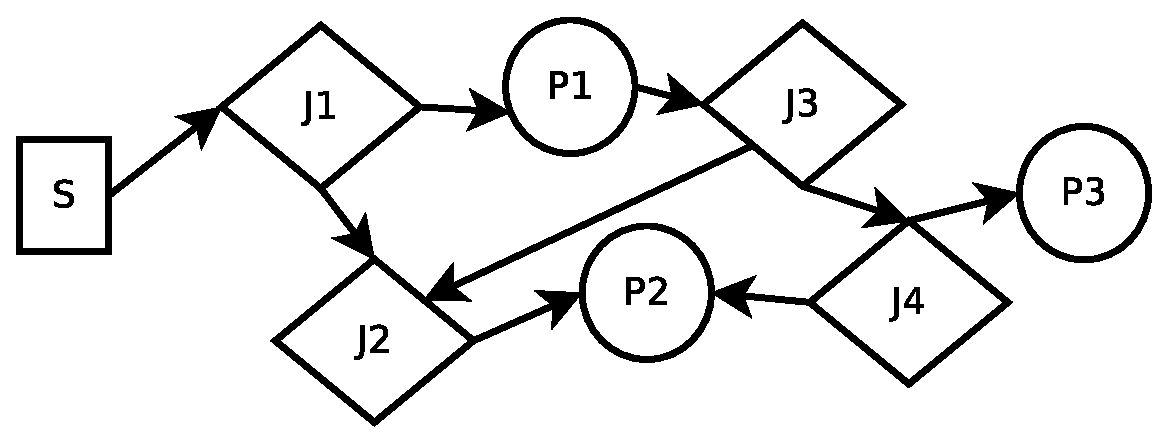
\includegraphics[width=8cm]{gnpbasic}
\caption{\label{gnpbasic} GNP Basic Implementation}
\end{center}
\end{figure}

\begin{figure}[tb]
\begin{center}
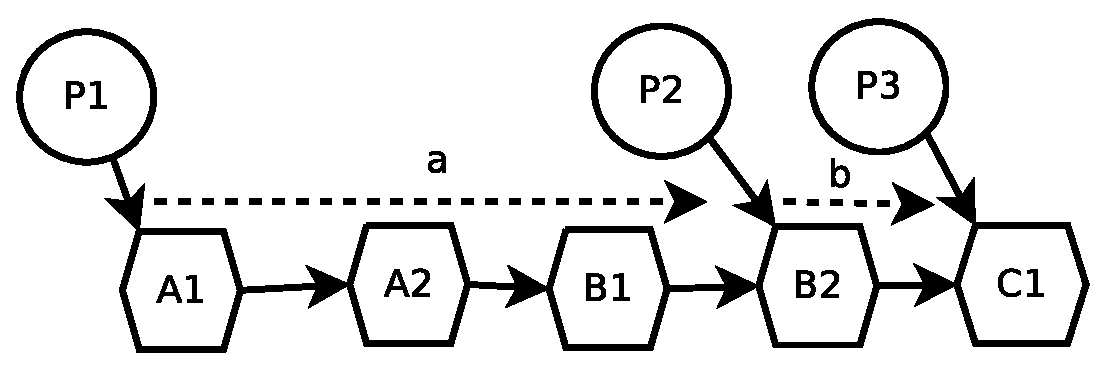
\includegraphics[width=8cm]{gnpdatamining}
\caption{\label{gnpdatamining} GNP Implementation on Data Mining}
\end{center}
\end{figure}

In this research, GNP is used to handle rule extraction from datasets by analyzing the records. Each judgement node of GNP represents an attribute with value range. For example, price attribute could be divided into three ranges (low, middle, high), and one range is assigned to one node in GNP. GNP makes rules by evolving combinations of nodes and measures the coverage of the extracted rules. Coverage means that how much data in a database each rule can represent (cover). Rules that pass the coverage threshold will be stored in the rule pool, then in the KP phase, the stored rules are distributed to several sites. The point of this paper is to distribute rules, not the data, which contributes to distributing any data into the sites considering the similarities between rules and data. The detailed explanation of the implementation of GNP in rule extraction is available in section 3.1.

\subsection{Knapsack Problem}
KP is a combinational optimization problem dealing with a set of items, each with a mass and a value, determining the number of each item to include in a collection so that the total weight is less than or equal to the given limit and the total value is as large as possible. KP is defined as follows.

\begin{eqnarray}
\begin{array}{lll}
\text{maximize}~St=\underset{i=1}{\overset{n}{\sum}}V_{i}x_{i}, \text{~~subject to~~~} \underset{i=1}{\overset{n}{\sum}}w_{i}x_{i}\leq W \\
\end{array}
\label{eq:ss}
\end{eqnarray}

$x_{i}$ = fragment $i$; $V_{i}$ = value (similarity to the leader rule) of fragment $i$; $w_{i}$ = weight (data size) of fragment $i$; W = capacity of the site.
By allowing each fragment (item) to be added more than once to sites (knapsack), this optimization can handle the problem of replication \cite{knapsack, knapsack2}.

In this research KP is used to handle a distribution of rules extracted by GNP to each site. Rules with high data coverage will be leaders of each site and KP will consider the similarity between the leader rules and remaining rules (which is considered as a value of item (rule) in KP) and coverage of rules (which is considered as weight in KP) should be matched with site capacities. Therefore, the similar rules to a certain leader are mainly put into the same site.
Detail explanation of the implementation of KP in the rule distribution is available in section 3.2.

\section{Combination of GNP and Knapsack problem}

Implementation for processing record clustering is separated into two parts: GNP rule extraction and KP rule distribution.

\subsection{GNP Rule Extraction}

GNP is used to extract rules from database by analyzing database structure including:
\begin{description}
\item [Attributes amount]: the number of attributes in a dataset. Each attribute will be spitted into some nodes depending on its variation and value ranges (distance of minimum value and maximum value). 
\item [Data amount]: the number of records in a dataset.
\item [Data variation]: how much different records are contained in a dataset. If every record in a dataset is different, variation is 100\%, if half of record in the dataset is different, variation is 50\%, and if every record in a dataset is the same, variation is $1/$(the number of data)$ \times 100\%$. For example in Table. \ref{frequency-table} there are six data variation in total 300 data, so variation will be $(6/300)\times100=2\%$.
\end{description}
The node preparation for GNP rule extraction contains two phases: node definition and node arrangement. In addition, two kinds of node arrangement methods are proposed: one is full random arrangement and the other is partial random arrangement.

\subsubsection{Node Definition}
Main purpose of node definition is to define nodes that will be combined to create rules. First step is to find the minimum and maximum value of each attribute. For example, the minimum value of ``price" attribute is 10 and the maximum value is 150 in the dataset with 300 records. Then, a frequency table is created per attribute as shown in Table \ref{frequency-table}. 
$x$ shows the price of a product, and $f$ shows how many times the product with the same price is recorded in the database. For example, product(s) with price $x=10$ appeared 30 times.
%In Table \ref{frequency-table}, the ``price" attribute is divided into three ranges. 
Mean $(\overline{xf})$ and standard deviation $S$ are calculated by Eq. \ref{eq:standarddeviation}, where $(\overline{xf})$ is used here and $S$ will be used in section 3.1.3. as spread measurement of attributes.

\begin{eqnarray}
\begin{array}{lll}
\overline{xf}=\frac{\sum xf}{\sum f}=75.42 \\
S=\sqrt{\frac{\sum(x-\overline{x})^{2}f}{\sum f}}=34.56
\end{array}
\label{eq:standarddeviation}
\end{eqnarray}

\begin{figure}[tb]
\begin{center}
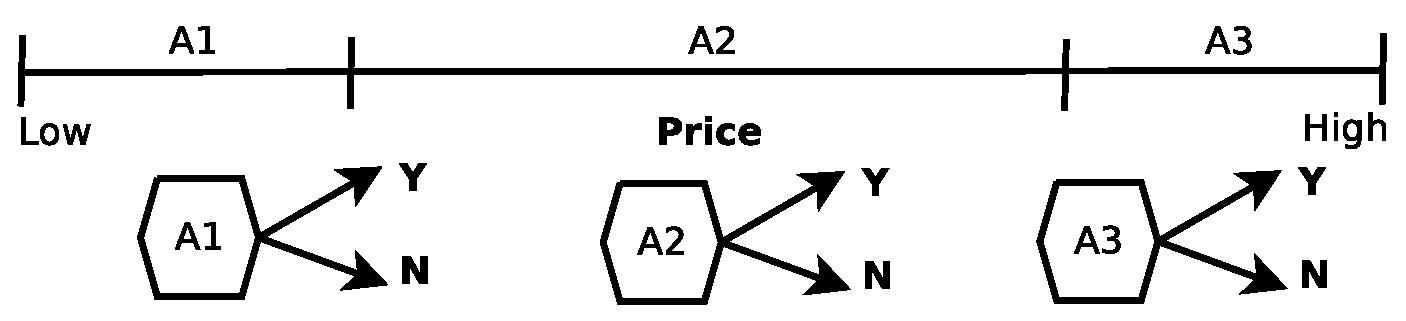
\includegraphics[width=8cm]{attributejudge}
\caption{\label{nodejudge} Node for judging attributes}
\end{center}
\end{figure}

To define nodes from Table \ref{frequency-table}, data should be divided equally based on data amount. For example, three nodes could be created by dividing value range into three ranges considering the occurrence frequency as shown in Fig. \ref{nodejudge}. In this example, three ranges are: $x = \left\{ 10,25,50 \right\} $ (75 data), $x = \left\{ 80 \right\} $ (140 data) and $x = \left\{ 100,150 \right\} $ (85 data). First node and third node contain more than one prices because each single record (10,25,50,100,150) does not have enough frequency to be defined as node. Mean ($\overline{xf}=75.42$) is used to measure the minimum frequency to become a node. Through the measurement, second node can created from single record ($x = \left\{ 80 \right\} $ with 140 data).

\begin{table}[tb]
\caption{\label{rule-example}Example of Single Rule with Four Attributes}
\begin{center}
\begin{tabular}{|c|c|c|c|}
\hline 
A1 & B3 & C2 & D1\tabularnewline
\hline 
5-9 & 30-50 & 40-79 & 1-4\tabularnewline
\hline 
\end{tabular}
\end{center}
\end{table}

\begin{table}[tb]
\caption{\label{dataset-example}Example of Dataset to be Covered}
\begin{center}
\begin{tabular}{|c|c|c|c|c|}
\hline 
A & B & C & D & match\tabularnewline
\hline 
8 & 12 & 56 & 1 & 3/4\tabularnewline
\hline 
6 & 45 & 45 & 2 & 4/4\tabularnewline
\hline 
2 & 23 & 43 & 2 & 2/4\tabularnewline
\hline 
\end{tabular}
\end{center}
\end{table}

Fitness function of extracted rule measured by its coverage. Coverage of rules measured by compare each attribute range to record on data set. Table. \ref{rule-example} shows example of extracted rule with four attributes and Table. \ref{dataset-example} shows example of dataset that used to be covered. Coverage threshold is used to determine passing status of records as covered or not. In this example, if coverage threshold is 3/4, data 1 and 2 are covered. Value of coverage threshold mostly increase the coverage rate of extracted rules but decrease the cluster quality.

\subsubsection{Node Arrangement : Full Random}
The purpose of node arrangement is to select necessary nodes for efficiently extracting a large number of rules. Full random method randomly selects nodes from the defined nodes in section 3.1.1 and makes graph structures. From the created graph structures, GNP extracts a large number of important rules and stores them in the rule pool (Fig. \ref{gnp_rulepool}). How to extract rules from the graph structures is described in \cite{gnp2} in detail.

\begin{figure}
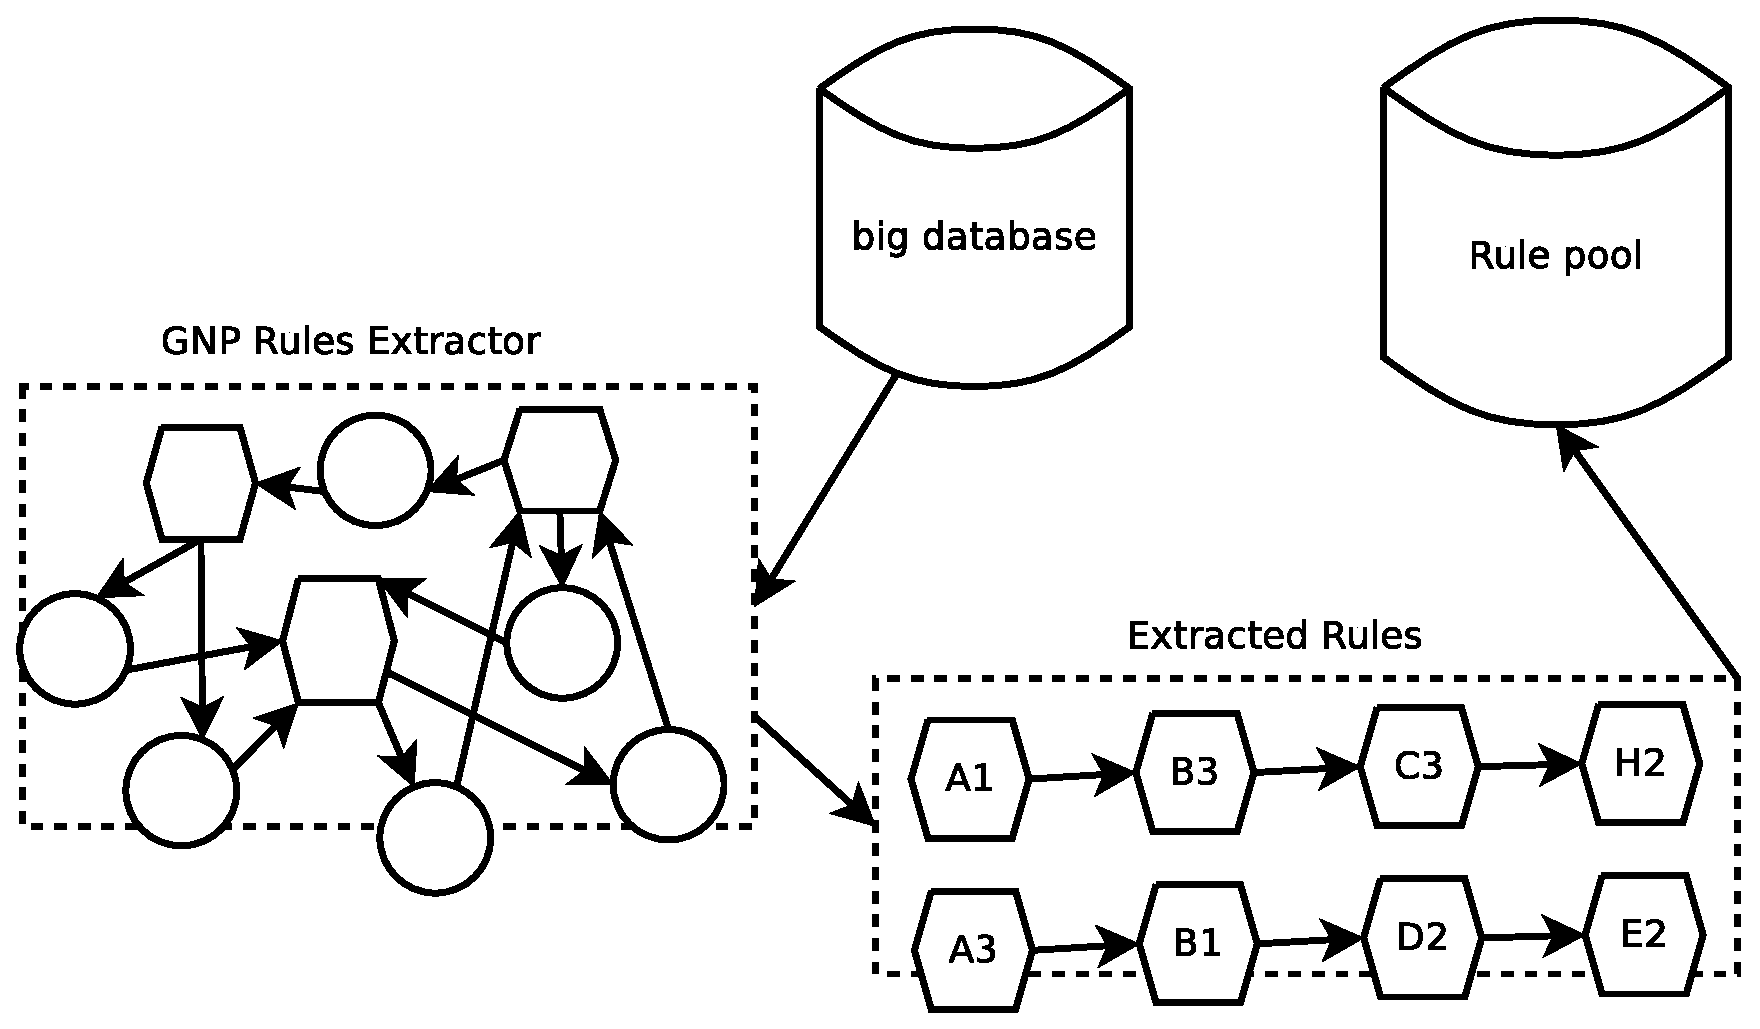
\includegraphics[width=8cm]{gnp_rulepool}
\caption{\label{gnp_rulepool} GNP rule extraction}
\end{figure}

After rules are extracted, GNP will measure the amount of coverage archived by the rules. In this research, coverage of rule {\it r} means the number of records that match (covered by) the rule {\it r}. If the coverage exceeds the coverage threshold, such rules will be added to rule pool, otherwise, the rules will be discarded. Rules with high coverage will be defined as elite rules and will be the leaders of each cluster (site) in KP process.

Rule extraction process will continue until :
\begin{itemize}
\item All data in the database are covered, and
\item Minimum amount of coverage of all rules are archived.
\end{itemize}

To create a large number of good rules, crossover and mutation are executed.
\begin{description}
\item [Crossover:] exchange one or more node(s) between parents to make new rules
\item [Mutation:] change one or more node(s) to make different combination of nodes
\end{description}
Crossover is effective to switch each weak nodes (nodes with less data frequency) of the parents with strong nodes (nodes with more data frequency). Mutation is effective to switch weak nodes of one individual to strong nodes.

\subsubsection{Nodes Arrangement : Partial Random}
As described in section 3.1.1, every attribute may have unbalanced frequency of data. Randomly combining different attributes results in decreasing the coverage. For example, in a database, there are 500 products that have a price around 50-100[USD], and 200 products in stationary category. 
However, suppose there are only five products that are matched with both conditions. In this case, ``price[USD] $\in$ [50,100]" and ``category = stationary" are a bad combined condition. On the other hand, if there is 100 products that are matched with condition of price[USD] $\in$ [1,10] and category = stationary, combining these conditions would make good rules.

To find a good arrangement, first, attributes with the low standard deviation (Eq. \ref{eq:standarddeviation}) are selected. 
Then, one or more nodes with the highest frequency $f$ of the selected attribute will be randomly connected as short rules (templates). 
If the combinations of these templates and other nodes produce good rules with high coverage, the templates are stored in the good arrangement set (Fig. \ref{newgnp}).
For example, in Table. \ref{frequency-table}, second node : $x$ = [80] (140 data) will be used in node arrangement as a high frequency node.

When initializing GNP structures, node arrangement with partial random method does not randomly prepare the nodes of attributes, but randomly prepare only a part of the nodes, and the remaining nodes are selected from good arrangement (combination) set to find much better combination of nodes (rules). 
As a result, GNP can extract rules with high coverage.

The objective of this method is to find general characteristics of data that is difficult to be found by full randomization. For example, most of stationary products have a price under 10[USD] and weight less than 100 grams. That would be general characteristics of stationary and other attributes such as size, color etc. may be varied but generally does not dominate the characteristics of stationary.

\begin{figure}
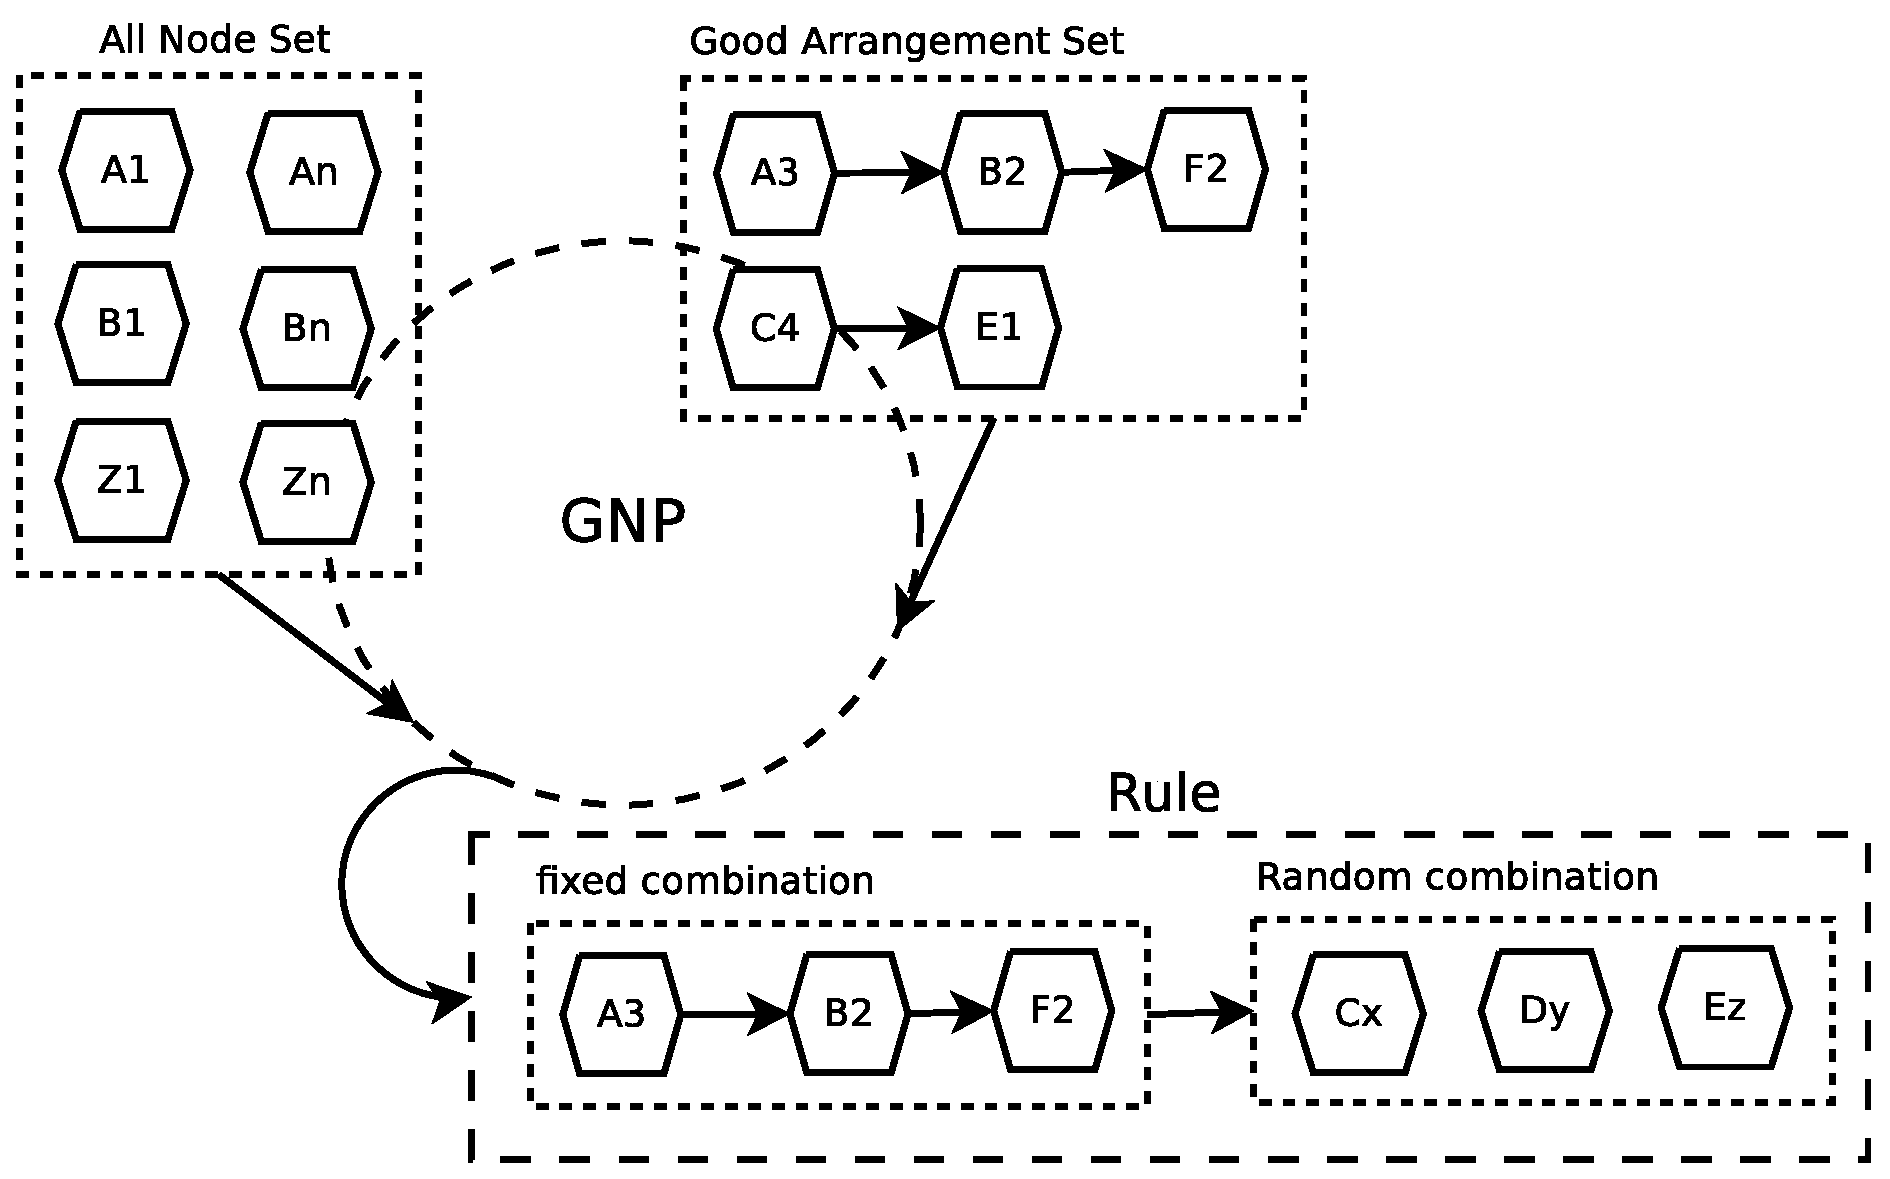
\includegraphics[width=8cm]{newgnp}
\caption{\label{newgnp} Node Arrangement Optimization in GNP}
\end{figure}

Table. \ref{partial-random-attribute-example} shows example of nodes with high amount of coverage. {\it Attribute} shown nodes name, alphabet describe attribute index and numeric describe range index. In example A1 and A2 are same attribute with different range which shown by different minimum{\it min} and maximum{\it Max} value. {\it S} shown standard deviation of each attribute. In example A1 and A2 have a same standard deviation because they are on same attributes.

\begin{table}[tb]
\caption{\label{partial-random-attribute-example}Example of Attribute to be Used on Partial Random}
\begin{center}
\begin{tabular}{|c|c|c|c|c|}
\hline 
Attribute & Min & Max & $S$ & Coverage\tabularnewline
\hline 
A2 & 149 & 246 & 36 & 28\tabularnewline
\hline 
B3 & 660 & 1626 & 48 & 75\tabularnewline
\hline 
A1 & 42 & 102 & 36 & 68\tabularnewline
\hline 
D3 & 1592 & 2340 & 47 & 30\tabularnewline
\hline 
\end{tabular}
\end{center}
\end{table}

In partial random method attributes with high amount of coverage will combined each other like shown in Table. \ref{partial-random-combination-example} and combination with high amount of coverage will be added in fixed combination set. As shown in Table. \ref{partial-random-combination-example2} three combination that have a coverage more than 20 is selected. To make a complete rule, fixed combination will randomized with remaining attributes that not included in fixed combination. In Table. \ref{partial-random-combination-example2}, when $A2\cap D3$ is selected, remaining attributes that will be randomized are B and C. In some case coverage can be zero although have used fixed combination of nodes with high coverage, because in dataset with random record there is not always contain every combination of value.

\begin{table}[tb]
\caption{\label{partial-random-combination-example}Example of Combination of Partial Random}
\begin{center}
\begin{tabular}{|c|c|c|c|c|}
\hline 
$x\cap y$ & A2 & B3 & A1 & D3\tabularnewline
\hline 
A2 & - & 18 & - & 22\tabularnewline
\hline 
B3 & 18 & - & 15 & 23\tabularnewline
\hline 
A1 & - & 15 & - & 21\tabularnewline
\hline 
D3 & 22 & 23 & 21 & -\tabularnewline
\hline 
\end{tabular}
\end{center}
\end{table}

\begin{table}[tb]
\caption{\label{partial-random-combination-example2}Example of Combination of Partial Random with Remaining Attributes}
\begin{center}
\begin{tabular}{|c|c|c|c|}
\hline 
GBS & RN1 & RN2 & Coverage\tabularnewline
\hline 
$A2\cap D3$ & B1 & C2 & 0\tabularnewline
\hline 
$A2\cap D3$ & B3 & C2 & 10\tabularnewline
\hline 
$A1\cap D3$ & B3 & C2 & 14\tabularnewline
\hline 
$B3\cap D3$ & A1 & C2 & 12\tabularnewline
\hline 
\end{tabular}
\end{center}
\end{table}

\subsection{Rule Distribution with Knapsack Problem}
After all the records in a dataset are covered by rules extracted by GNP, KP is used to distribute rules to several sites. Rules with high coverage (elite) will be the leaders of each site, then KP will consider the similarity of the remaining rules to the leader rules (value) and coverage of the rules (weight) in order to distribute the remaining rules to the sites. This process is shown in Fig. \ref{knapsack}

\begin{figure}[tb]
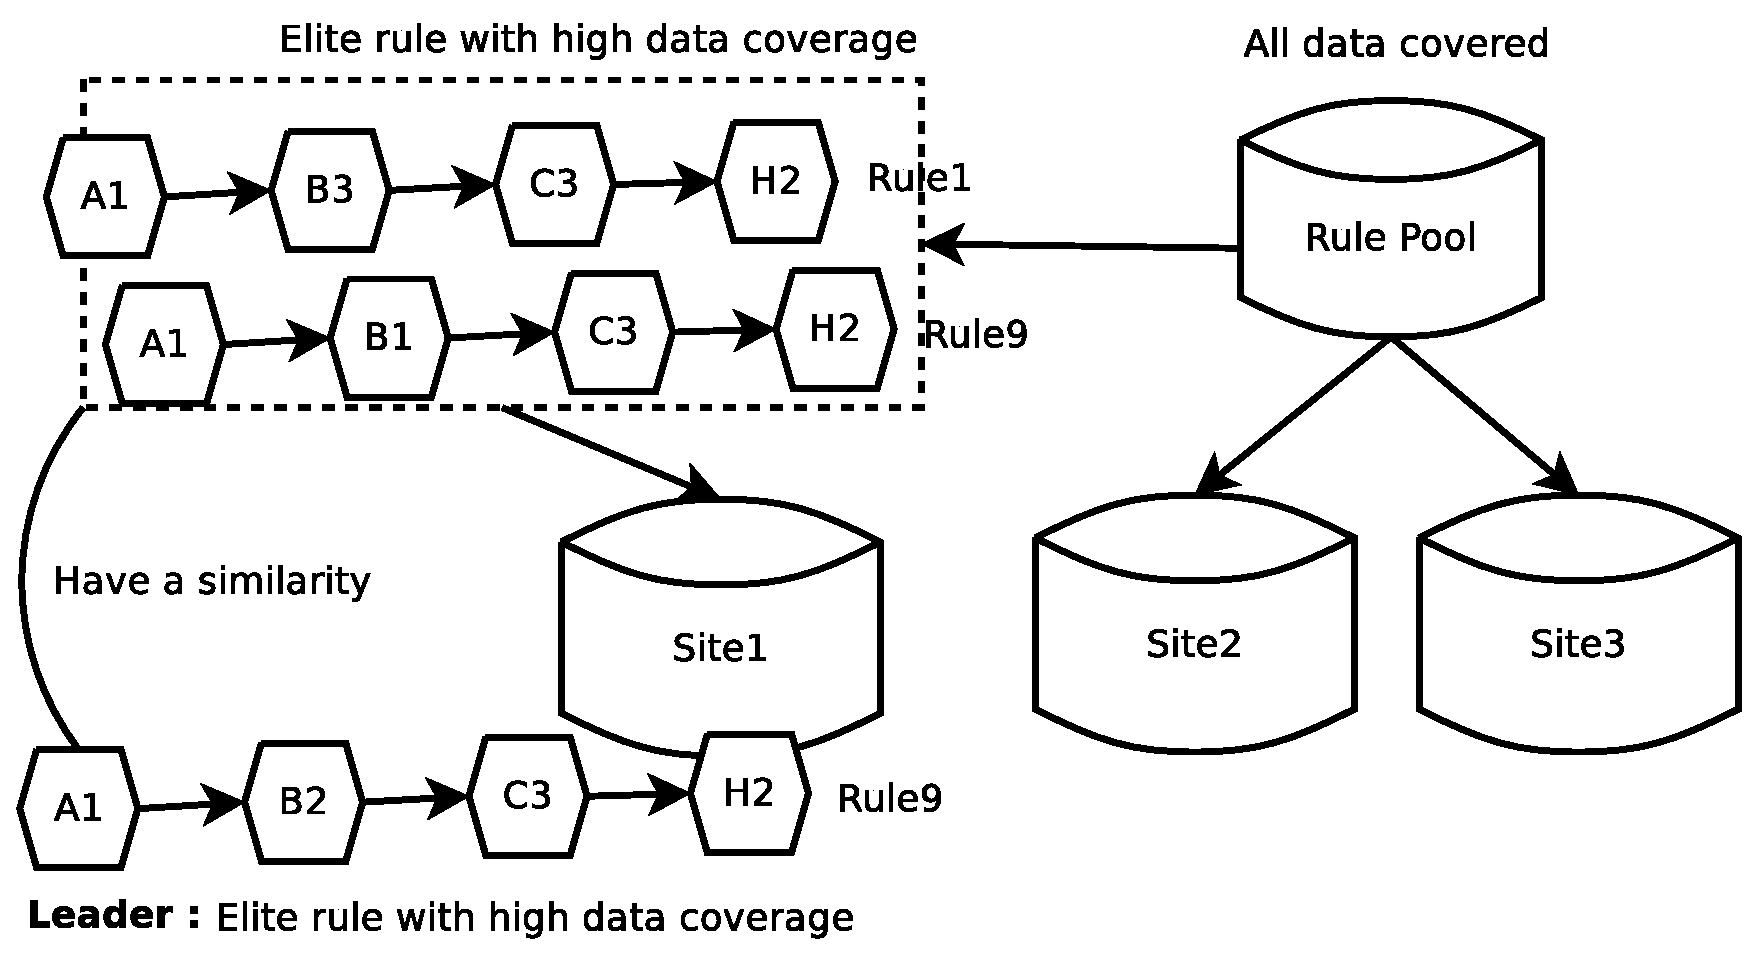
\includegraphics[width=8cm]{knapsack}
\caption{\label{knapsack} Rule Distribution with Knapsack Problem}
\end{figure}

Euclidean distance (Eq. \ref{euclidean-distance}) \cite{euclidean-distance} is used to measure distance between remaining rule ($P$) and leader rule ($Q$) in each site. 

\begin{eqnarray}
\begin{array}{lll}
d(P,Q)=\sqrt{\underset{i}{\sum}(p_{i}-q_{i})^{2}} \\
\qquad\quad=\sqrt{(p_{1}-q_{1})^{2}+...+(p_{n}-q_{n})^{2}}, \\
\end{array}
\label{euclidean-distance}
\end{eqnarray}
where,

\begin{description}
\item [${p_{i}}$] : value of attribute $i$ contained in remaining rule $P$,
\item [${q_{i}}$] : value of attribute $i$ contained in leader rule $Q$,
\item [${n}$] : number of attributes.
\end{description}

The values of each attribute are normalized to be the same standard in the distance calculation. For example Table. \ref{attributes-list} shows nodes of each attribute with its ranges and distance. Last row shows total distance of each attribute. Table. \ref{remained-rules} shows remained rules to be compared with leader rule which shown in \ref{rule-example}. {\it dist} shows number of attributes that have a distance from leader rule which if node is in same range its will counted just as zero. Calculation of euclidean distances shown on \ref{euclidean-distance-calculation}. If distance threshold is 60\% but site capacity is just two records, only two rules with lowest euclidean distance will be added to site which in example are rule two and three. Rule one will be added to another site which possibly meet with leader rule that have a lower distance than current site. 
%Table. \ref{euclidean-distances} shows an example of one remaining rule and leader rule. Distance is calculated based on sum of the difference between the same %attribute ($A,B,C,\dots$). 
%In Table \ref{euclidean-distances}, 
%If the leader rule and remaining rule have the same node (A1) on attribute A, thus the distance of attribute A is zero. However, the nodes of other attributes (B, C) %are different. 

%\begin{table}[tb]
%\vspace{1em}
%\caption{\label{euclidean-distances}Example of Rules}
%\begin{tabular}{|c|c|c|c|c|c|c|c|c|c|}
%\hline 
% & A1 & A2 & A3 & B1 & B2 & B3 & C1 & C2 & C3\tabularnewline
%\hline 
%$P$ & 1 & 0 & 0 & 0 & 1 & 0 & 0 & 0 & 1\tabularnewline
%\hline 
%$Q$ & 1 & 0 & 0 & 0 & 0 & 1 & 0 & 1 & 0\tabularnewline
%\hline 
%\end{tabular}
%\end{table}

\begin{table}[tb]
\caption{\label{attributes-list}Nodes of Each Attribute with its Range and Distance}
\begin{tabular}{|c|c|c|c|c|}
\hline 
 & A & B & C & D\tabularnewline
\hline 
1 & {[}5,9{]};5 & {[}5,19{]};15 & {[}10,39{]};30 & {[}1,4{]};4\tabularnewline
\hline 
2 & {[}10,13{]};4 & {[}20,29{]};10 & {[}40,79{]};40 & {[}5,8{]};4\tabularnewline
\hline 
3 & {[}14,20{]};7 & {[}30,50{]};21 & {[}80,100{]};21 & {[}9,10{]};2\tabularnewline
\hline 
 & 16 & 46 & 91 & 10\tabularnewline
\hline 
\end{tabular}
\end{table}

\begin{table}[tb]
\caption{\label{remained-rules}Remained Rules}
\begin{center}
\begin{tabular}{|c|c|c|c|c|c|c|}
\hline 
Rule & A & B & C & D & dist & ED(\%)\tabularnewline
\hline 
1 & A1 & B2 & C1 & D2 & 2 & 54.71\tabularnewline
\hline 
2 & A2 & B3 & C2 & D1 & 1 & 31.25\tabularnewline
\hline 
3 & A1 & B1 & C2 & D1 & 1 & 32.61\tabularnewline
\hline 
\end{tabular}
\end{center}
\end{table}

\begin{eqnarray}
\begin{array}{lllllllll}
Rule1:((B3-B2)/B)+((C2-C1)/C) \\ 
\qquad\quad\,\,\,=10/46+30/91 \\ 
\qquad\quad\,\,\,=21.74\%+32.97\%=54.71\% \\
\qquad\quad\,\,\,=54.71\% \\
Rule2:((A2-A1)/A) \\
\qquad\quad\,\,\,=5/16 \\
\qquad\quad\,\,\,=31.25\% \\
Rule3:((B3-B1)/B) \\
\qquad\quad\,\,\,=15/46 \\
\qquad\quad\,\,\,=32.61\% \\
d(P,Q)=\sqrt{54.71^{2}+31.25{}^{2}+32.61^{2}} \\
\qquad\quad\,\,\,=70.94
\end{array}
\label{euclidean-distance-calculation}
\end{eqnarray}

In some cases, there is no large distance or almost the same distance between clusters. Such cases happen depending on the site capacities and distance between leader rules. If similar data cannot be included in one site due to the limitation of capacity, the remaining data will be distributed in a new site or another site that still has a space.

\section{Simulations}
First, full random and partial random methods in the rule extraction of GNP are compared. Then, knapsack rule distribution is carried out and its results are compared with k-means and hierarchical clustering.

\subsection{GNP Rule Extraction}
The coverage of rules and the number of extracted rules depend on the complexity of a dataset. Examples are shown in Figs. \ref{affectedcoverage2014-02-13-11-53-24} and \ref{affectedcoverage2014-02-13-11-45-04}. The horizontal axis shows the rule numbers, and the vertical axis shows the coverage of each rule. In the simple dataset with less data variation (Fig. \ref{affectedcoverage2014-02-13-11-53-24}), maximum value of coverage reaches around 40. But some rules cover only one--two records. Such situation occurs when some data have unique values and are difficult to be covered by general rules. Fig. 7 shows the coverage of each rule when the dataset is complicated, where the maximum coverage is nine. Therefore, more rules are necessary to cover all the records in the complicated dataset.

\begin{figure}[tb]
\includegraphics[width=8cm]{coverage-simple}
\caption{\label{affectedcoverage2014-02-13-11-53-24} Coverage of the simple dataset}
\end{figure}
\begin{figure}[tb]
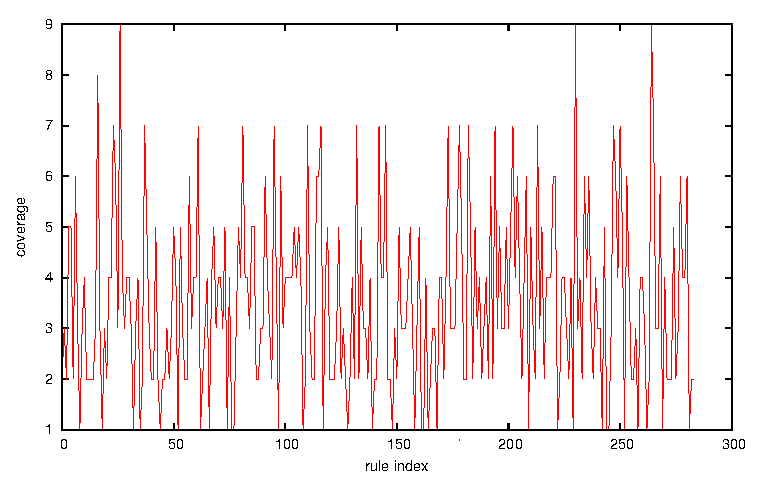
\includegraphics[width=8cm]{coverage-complex}
\caption{\label{affectedcoverage2014-02-13-11-45-04} Coverage of the complicated dataset}
\end{figure}

Figs. \ref{coverage2014-02-13-11-53-24} and \ref{coverage2014-02-13-11-45-04} show the number of extracted rules v.s. coverage. When the dataset is simple as Fig. \ref{coverage2014-02-13-11-53-24}, 250 extracted rules can cover all the 1,000 data in a dataset, i.e., 100\% coverage. However, when the dataset is complicated as Fig. \ref{coverage2014-02-13-11-45-04}, around 400,000 rules are needed to cover all data. 
The coverage increases rapidly at the beginning of rule extraction but more slowly towards the end. It means that the records that have been already covered by previously extracted rules are not recovered by another rule. Therefore, the remaining data gradually become difficult to be covered.  

\begin{figure}[tb]
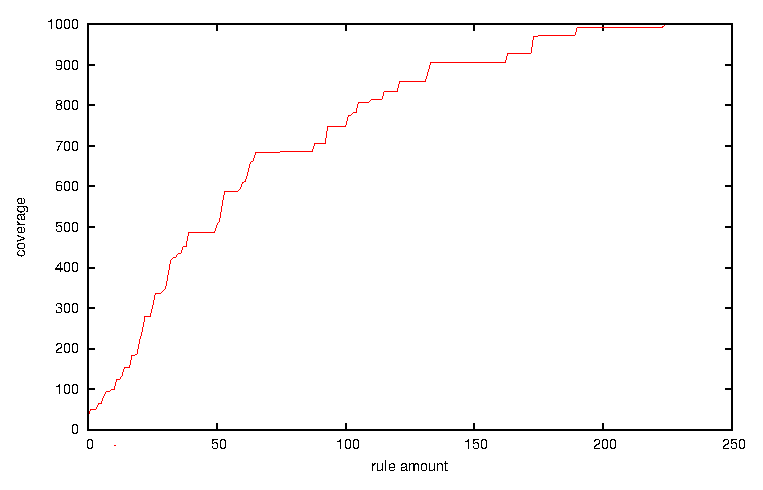
\includegraphics[width=8cm]{coveragerule-simple}
\caption{\label{coverage2014-02-13-11-53-24} Relation between the number of extracted rules and coverage in the simple dataset}
\end{figure}
\begin{figure}[tb]
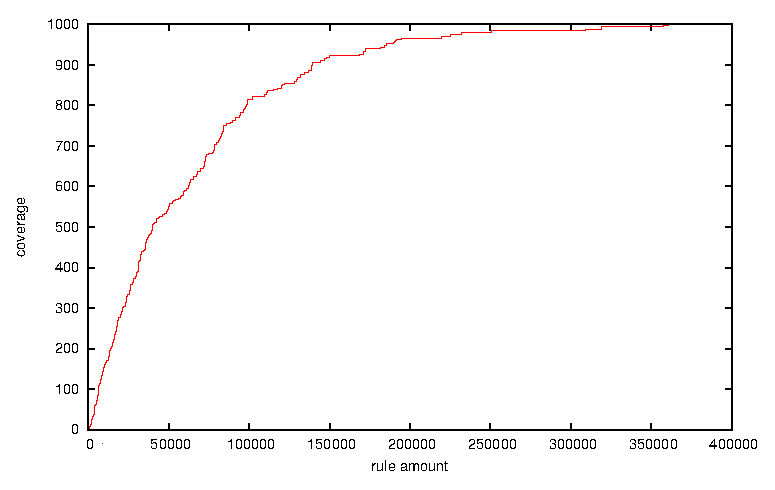
\includegraphics[width=8cm]{coveragerule-complex}
\caption{\label{coverage2014-02-13-11-45-04} Relation between the number of extracted rules and coverage in the complicated dataset}
\end{figure}

Result comparison between two node arrangement methods, that is, full randomization and partial randomization, are shown in Tables \ref{gnp-rule-extraction-result-full}. Six datasets are used for comparison, where the number of data and data variation are different. The performance evaluation is executed based on the iterations needed to cover all the data, the number of rules covering the data, and coverage value. Here, iteration means one time rule extraction.
When the number of attributes and data variation are increased, the number of iterations needed to cover all the data tends to be increased. However, comparing the iteration needed by full randomization and partial randomization, partial randomization shows better results, i.e., less iteration are needed. The number of rules obtained by both methods are not different so much, but coverage obtained by partial randomization show better result because it can create good combinations of attributes (nodes).

\subsection{Knapsack Rule Distribution}
Here, silhouette value (Eq. \ref{eq:silhouette}) is used to evaluate the clustering results. Silhouette provides a succinct graphical representation of how well each object lies within its cluster \cite{silhouette}.

\begin{eqnarray}
\begin{array}{lll}
s = \frac{b - a}{\max\{a,b\}} \\
\quad= \begin{cases} 1-a/b, & \mbox{if } a < b \\ 0, & \mbox{if } a = b \\ b/a-1, & \mbox{if } a > b \\ \end{cases} 
\end{array}
\label{eq:silhouette}
\end{eqnarray}
\begin{description}
\item [s:] Silhouette value for a single sample. The Silhouette value for a set of samples is given as the mean of the Silhouette values of each sample.
\item [a:] mean distance between a sample and all other points in the same cluster.
\item [b:] mean distance between a sample and all other points in the second nearest cluster.
\end{description}

The results of rule distribution are shown in Table. \ref{knapsack-result}.
%\begin{description}
$k$ is the number of clusters (sites).
``Size of Each Site" shows the capacity of each site. For example, 1:1:1:1 means all the four sites have a same size, and 1:4:2:1 means that the second site (size four) is four time larger capacity than the first site (size one).
``Average, Max and Min" show the data on Silhouette values obtained by generated clusters.
%\end{description}

\begin{table*}[tb]
\caption{\label{gnp-rule-extraction-result-full}Results of GNP rule extraction with full randomization in six datasets}
\begin{center}
\begin{tabular}{|l|l|l|l|l|l|l|l|l|}
\hline 
\multicolumn{3}{|l|}{} & \multicolumn{3}{c|}{Full Random} & \multicolumn{3}{c|}{Partial Random}\tabularnewline
\hline 
Attribute & Data & Variation & Iteration & Rule & Coverage & Iteration & Rule & Coverage\tabularnewline
\hline 
3 & 1000 & 50.00\% & 410 & 62 & 15.87 & 93 & 61 & 16.84\tabularnewline
\hline 
3 & 10000 & 20.00\% & 431 & 29 & 344.82 & 121 & 27 & 367.24\tabularnewline
\hline 
8 & 1000 & 30.00\% & 458192 & 39 & 26.64 & 387293 & 39 & 26.64\tabularnewline
\hline 
8 & 10000 & 60.00\% & 512239 & 70 & 145.89 & 435729 & 69 & 153.56\tabularnewline
\hline 
15 & 1000 & 70.00\% & 98245k & 76 & 13.15 & 98189k & 72 & 14.67\tabularnewline
\hline 
15 & 10000 & 10.00\% & 2678k & 15 & 62.57 & 2537k & 12 & 67.38\tabularnewline
\hline 
\end{tabular}
\par\end{center}
\vspace{1em}
\end{table*}

\begin{table}[tb]
\caption{\label{knapsack-result}Result of Knapsack Problem (Silhouette values)}
%\begin{flushleft}
\begin{tabular}{|l|l|l|l|l|}
\hline 
$k$ & Size of Each Site & Average & Max & Min\tabularnewline
\hline 
4 & 1:1:1:1 & 0.98 & 0.99 & 0.95\tabularnewline
\hline 
4 & 1:4:2:1 & 0.95 & 0.99 & 0.87\tabularnewline
\hline 
6 & 1:1:1:1:1:1 & 0.96 & 0.99 & 0.91\tabularnewline
\hline 
6 & 1:5:2:6:3:2 & 0.94 & 0.99 & 0.86\tabularnewline
\hline 
8 & 1:1:1:1:1:1:1:1 & 0.94 & 0.98 & 0.88\tabularnewline
\hline 
8 & 4:2:4:6:4:2:7:5 & 0.89 & 0.98 & 0.79\tabularnewline
\hline 
\end{tabular}
%\par\end{flushleft}
\end{table}

\subsection{Comparison with K-means and Hierarchical Clustering}
Clustering methods that will be used for the comparison are k-means and hierarchical clustering because both of the methods also use euclidean distance. K-means is based on a centroid concept for cluster separation and the centroids also represent each cluster. Hierarchical clustering is selected for comparison because similar concept to the proposed method using leader rules is used to distribute rules.
Although both methods can set the number of clusters to be created, they does not have a function to measure cluster capacity as KP. Thus, cluster capacity problem is not discussed in this comparison.
The features of attributes contained in the dataset for comparison is shown in Table \ref{dataset-used-to-comparison}. 
In this simulation, eight datasets are prepared, where the values of each record are determined randomly in the ranges of each attribute,
and the number of records and record variation are different.

\begin{table}[tb]
\vspace{1em}
\caption{\label{dataset-used-to-comparison}Value ranges of attributes in the dataset}
\begin{center}
\begin{tabular}{|l|l|l|l|}
\hline 
Attribute & Min Value & Max Value\tabularnewline
\hline 
1 & 100 & 500\tabularnewline
\hline 
2 & 1000 & 2000\tabularnewline
\hline 
3 & 700 & 1500\tabularnewline
\hline 
4 & 1 & 5\tabularnewline
\hline 
5 & 15 & 95\tabularnewline
\hline 
6 & 10000 & 30000\tabularnewline
\hline 
7 & 5000 & 50000\tabularnewline
\hline 
8 & 1 & 10\tabularnewline
\hline 
\end{tabular}
\par\end{center}
\end{table}

Table \ref{silhouette-comparison} shows more information on the eight datasets (including simple and complicated datasets) and Silhouette values obtained by the proposed method (GNP-KP), K-means and hierarchical clustering (HC). 
Fig. \ref{silhouette2014-02-13-11-45-04} graphically shows the silhouette values. When the number of attributes is small, 
the values obtained by GNP-KP and K-means are almost the same and higher than HC, however as the number of attributes increases, K-means shows lower values and HC shows higher values than K-means. GNP-KP shows the highest values in all the cases.

\begin{table}[tb]
\caption{Data on Silhouette values in the eight cases}
\label{silhouette-comparison}
%\begin{center}
\begin{tabular}{|l|l|l|l|l|l|l|}
\hline 
$k$ & attr & data & var & K-mean & HC & GNP-KP\tabularnewline
\hline 
2 & 2 & 1000 & 30 & 0.981 & 0.873 & 0.982\tabularnewline
\hline 
8 & 2 & 5000 & 50 & 0.963 & 0.871 & 0.972\tabularnewline
\hline 
2 & 4 & 1000 & 30 & 0.885 & 0.790 & 0.927\tabularnewline
\hline 
8 & 4 & 5000 & 70 & 0.793 & 0.648 & 0.915\tabularnewline
\hline 
6 & 8 & 3000 & 30 & 0.476 & 0.591 & 0.784\tabularnewline
\hline 
8 & 8 & 10000 & 50 & 0.402 & 0.579 & 0.730\tabularnewline
\hline 
3 & 10 & 1000 & 30 & 0.345 & 0.559 & 0.666\tabularnewline
\hline 
8 & 10 & 5000 & 70 & 0.302 & 0.500 & 0.656\tabularnewline
\hline 
\end{tabular}
$k$: the number of clusters, attr: the number of attributes, var: variation[\%]
\vspace{1em}
%\par\end{center}
\end{table}

\begin{figure}
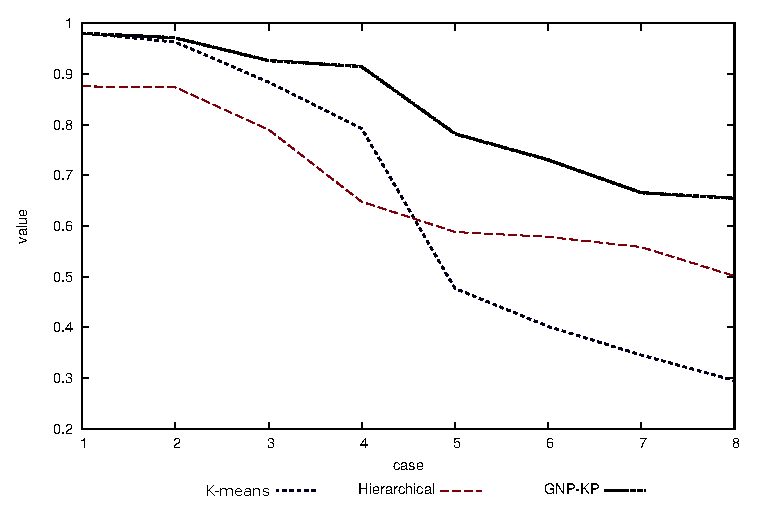
\includegraphics[width=8cm]{silhoutte}
\caption{\label{silhouette2014-02-13-11-45-04} Comparison of Silhouette values in eight cases}
\end{figure}

Log of GNP result explained by Table. \ref{extracted-nodes-and-its-coverage}, \ref{nodes-substances-on-each-sites} and \ref{good-combination-result}. Table. \ref{extracted-nodes-and-its-coverage} shows nodes of each attribute which separated into three ranges and its coverage. Each attributes shows unbalanced coverage by each ranges. For example attribute F dominated with data with range between 11573 and 14458. This domination effects to attributes substances on each site(cluster) which shown by \ref{nodes-substances-on-each-sites}. Site with larger capacity contain more nodes variation of rule and data. There is no site that contain only one variation of rule. Its shown by always more than one variation of ranges for one attribute on each site. For example site 1 contain both of H1 and H2, so its possible to have a two variation of rule.

As described on section 3.1.3 about partial random, combination attribute range with high coverage also resulting high coverage. But because each site(cluster) have a limit of capacity, attribute range with high coverage become subtances of most sites or can be whole sites. Because high data amount difficult to be fit in one site's capacity, so remaining data will be distributed to other site. This case could be decreased by increase amount of attribute range, so its will decrease the range domination but its will increase calculation amount and impact to proccesing time. 

\begin{table*}[tb]
\caption{\label{extracted-nodes-and-its-coverage}Extracted Nodes and Its Coverage}
\begin{center}
\begin{tabular}{|l|l|l|l|l|l|l|}
\hline 
 & \multicolumn{2}{l|}{1} & \multicolumn{2}{l|}{2} & \multicolumn{2}{l|}{3 }\tabularnewline
\hline 
A & {[}164,227{]} & 160 & {[}284,357{]} & 583 & {[}381,500{]} & 257\tabularnewline
\hline 
B & {[}1129,1269{]} & 522 & {[}1456,1574{]} & 173 & {[}1651,2000{]} & 305\tabularnewline
\hline 
C & {[}791,849{]} & 418 & {[}892,897{]} & 10 & {[}1020,1500{]} & 572\tabularnewline
\hline 
D & {[}1,1{]} & 135 & {[}2,2{]} & 499 & {[}3,5{]} & 366\tabularnewline
\hline 
E & {[}20,23{]} & 148 & {[}31,44{]} & 631 & {[}44,95{]} & 221\tabularnewline
\hline 
F & {[}11573,14458{]} & 687 & {[}14569,15814{]} & 184 & {[}19105,30000{]} & 129\tabularnewline
\hline 
G & {[}9898,10418{]} & 304 & {[}17664,21672{]} & 637 & {[}30634,50000{]} & 59\tabularnewline
\hline 
H & {[}1,1{]} & 244 & {[}2,2{]} & 264 & {[}2,10{]} & 492\tabularnewline
\hline 
\end{tabular}
\end{center}
\end{table*}

Partial random created by combining nodes with high coverage which on average of coverage exceeds 500. Result of fixed combination shown by Table. \ref{extracted-nodes-and-its-coverage}. Support means ratio of combination to the whole six site. For example combination $C3\cap E2\cap F1\cap G2$ available on every site so support are 100\% and combination $B1\cap E2\cap F1\cap G2$ available on five site so support is $5/6 = 83\%$. This feature could be used to explore patterns domination of records on dataset.

\begin{table*}[tb]
\caption{\label{nodes-substances-on-each-sites}Nodes Substances On Each Site}
\begin{center}
\begin{tabular}{|c|l|c|c|}
\hline 
Site & Attributes & Capacity & Data\tabularnewline
\hline 
1 & \{A2,B1,C3,D2,D3,E2,F1,G2,H1,H2\} & 100 & 69\tabularnewline
\hline 
2 & \{A1,A2,B1,B3,C2,C3,D2,D3,E1,E2,F1,G1,G2,H3\} & 500 & 209\tabularnewline
\hline 
3 & \{A3,C3,D2,D3,E2,F1,F2,G1,G2,H1,H2\} & 200 & 94\tabularnewline
\hline 
4 & \{A1,A2,B1,B3,C1,C3,D2,D3,E1,E2,E3,F1,F2,G2,G3,H1,H3\} & 600 & 420\tabularnewline
\hline 
5 & \{A3,B1,C3,D1,D3,E1,E2,F1,F3,G2,G3,H1,H2\} & 300 & 159\tabularnewline
\hline 
6 & \{A2,B1,B2,C1,C3,D1,D3,E1,E2,F1,F2,G1,G2,H2,H3\} & 200 & 49\tabularnewline
\hline 
\end{tabular}
\end{center}
\end{table*}

\begin{table}[tb]
\caption{\label{good-combination-result}Most Contained Node Arrangement on Sites}
\begin{center}
\begin{tabular}{|c|c|}
\hline 
Combination & Support(\%)\tabularnewline
\hline 
$C3\cap E2\cap F1\cap G2$ & 100\tabularnewline
\hline 
$B1\cap E2\cap F1\cap G2$ & 83\tabularnewline
\hline 
$A2\cap E2\cap F1\cap G2$ & 67\tabularnewline
\hline 
$E2\cap F1\cap G2\cap H2$ & 67\tabularnewline
\hline 
\end{tabular}
\end{center}
\end{table}

\section{Conclusions}
This paper proposes novel clustering method combining Genetic Network Programming and Knapsack Problem to handle a record clustering. The proposed method can find  good combinations of attributes to create rules for clustering, and also consider the capacity of sites to distribute rules. From the simulation results, the proposed method shows better clustering ability than K-means and hierarchical clustering in eight kinds of datasets. In the future, we will consider the replication problems of distributed databases, where the query frequency is considered in the clustering problems and frequently accessed data will be stored in several sites to decrease the load of the accesses.

%%%%%%%%%%%%%%%%% BIBLIOGRAPHY IN THE LaTeX file !!!!! %%%%%%%%%%%%%%%%%%%%%%
\begin{thebibliography}{9}

\bibitem{recordclustering}
Guinepain, S., Gruenwald, L., ``Automatic Database Clustering Using Data Mining'', {\it 17th International Conference on Database and Expert Systems Applications (DEXA'06)}, 
2006.

\bibitem{horizontalfragmentation}
P.R.Bhuyar, A.D.Gawande, A.B.Deshmukh, ``Horizontal Fragmentation Technique in Distributed Database'' {\it The International Journal of Scientific and Research Publications}, 2012.

\bibitem{horizontalfragmentation2}
Sanjay Agrawal, V. Narasayya, B. Yang, ``Integrating Vertical and
Horizontal Partitioning into Automated Physical Database Design'',
{\it SIGMOD}, June 2004.

\bibitem{gnp1}
Shingo Mabu, Ci Chen, Nannan Lu, Kaoru Shimada,
and Kotaro Hirasawa, ``An Intrusion-Detection Model Based on Fuzzy Class-Association-Rule Mining Using Genetic Network Programming'',
{\it IEEE Transactions On Systems, Man, And Cybernetics}, Vol. 41, No. 1, pp. 130-139, 2011.

\bibitem{gnp2}
Kaoru Shimada, Kotaro Hirasawa and Junglu Hu, Genetic Network Programming with Acquisition Mechanism of Association Rules, Journal of Advanced Computational Intelligence and Intelligence Informatics, Vol. 10, No. 1 pp. 102-111, 2006

\bibitem{knapsack}
Jiangfei Zhao; TingLei Huang; Fei Pang; Yuanjie Liu, ``Genetic Algorithm Based on Greedy Strategy in the 0-1 Knapsack Problem,'' {\it Genetic and Evolutionary Computing, 2009. WGEC '09. 3rd International Conference on , vol., no., pp.105,107}, 14-17 Oct. 2009

\bibitem{knapsack2}
Singh, R.P., ``Solving 01 Knapsack problem using Genetic Algorithms'', {\it Communication Software and Networks (ICCSN), 2011 IEEE 3rd International Conference on , vol., no., pp.591,595}, 27-29 May 2011

%\bibitem{customer2}
%Ishigaki, T.; Takenaka, T.; Motomura, Y., ``Computational Customer Behavior Modeling for Knowledge Management with an Automatic Categorization Using Retail Service's %Datasets'', {\it e-Business Engineering (ICEBE), 2010 IEEE 7th International Conference on , vol., no., pp.528,533}, 10-12 Nov. 2010

\bibitem{euclidean-distance}
Elizondo-Leal, J.C.; Ramirez-Torres, G., ``An Exact Euclidean Distance Transform for Universal Path Planning'', {\it Electronics, Robotics and Automotive Mechanics Conference (CERMA), 2010 , vol., no., pp.62,67}, Sept. 28 2010-Oct. 1 2010

\bibitem{silhouette}
Yanchi Liu, Zhongmou Li, Hui Xiong, Xuedong Gao, Junjie Wu, ``Understanding of Internal Clustering Validation Measures Yanchi'',
{\it IEEE International Conference on Data Mining}, 2010.

\end{thebibliography}

\end{document}
